\section{Results}\label{sec:results}

\subsection{When conversion raises the total as capital land declines}\label{sec:mask}

For a given capital-land quality level $q$, its annual contribution per hectare, $\Ups(q)$, is a concave quadratic. It peaks at $q^*=q_{\max}/2$; with the baseline parameters, the maximum is $0.066$\,gha\,ha$^{-1}$. The quality-related term contributes $0.016$ of that value, while direct yield contributes $0.05$\,gha\,ha$^{-1}$; the direct-yield component is larger in this case.

Conversion changes the aggregate according to the gap between the annual account contribution of one fast-land hectare and the effective value of one capital-land hectare. We call this gap the \emph{composition diagnostic}:
\begin{equation}\label{eq:dconv}
\dconv(q,D)=b_f(D)-\Ups(q).
\end{equation}
At baseline, $\dconv$ equals $+0.787$, $+0.784$, and $+0.794$\,gha\,ha$^{-1}$ at $q=0.3$, $0.6$, and $0.9$. Each lies in the composition-premium regime ($\dconv>0$), where conversion adds to the aggregate at the margin. At $\dconv=0$ the contribution is first-order neutral; below zero, it is a composition-discount. These labels describe the conversion term only. Maintenance, retirement, quality change, and other flows still determine the net change in $B$. At any given quality level, that contribution changes linearly with $A_c$; it has no interior maximum with respect to area.

\begin{proposition}[Conversion, aggregate change, and what the total can reveal]\label{prop:mask}
Let $T_b\equiv0$, $R_{rc}\equiv0$ and hold $D$ fixed, so that $b_f$ is constant. Along any solution of \eqref{eq:B}--\eqref{eq:q},
\begin{equation}\label{eq:identity}
\dot B=\dconv(q)\,u_c+b_f\big(\mu A_r-\eta_f A_f\big)+b_{G,c}\,G_c'(q)\,A_c\,\dot q .
\end{equation}
\begin{enumerate}[label=(\roman*)]
\item During conversion ($u_c>0$), $A_c$ falls when restoration is off. The conversion component of $\dot B$ is $\dconv(q)u_c$, positive exactly when $\dconv(q)>0$. It determines the sign of net $\dot B$ only if maintenance balances retirement ($\mu A_r=\eta_fA_f$) and quality is unchanged ($\dot q=0$).
\item In the reduced comparison—with fixed demand and debt, baseline availability shares, balanced maintenance and retirement, and no quality change—a positive $\dconv$ makes the shortfall shrink during conversion. The shortfall closes if the balance point is reached before the area floor binds. If the floor binds first, $A_c$ approaches $\Acmin$ and a shortfall may persist. Other active terms in the full model can change this result.
\item At fixed $b_f>0$ and $q$, $B=b_fA_f+\Ups(q)A_c$ supplies one equation for the two land areas. Near an interior state, a small change in $A_c$ can be offset by $\delta A_f=-(\Ups/b_f)\delta A_c$ and $\delta A_r=-\delta A_f-\delta A_c$, preserving both $B$ and total area as long as the land bounds are respected. Thus several nearby allocations can have the same $B$; the aggregate alone does not identify $A_c$. For a finite observed change $\Delta B$, the offset is $\Delta A_f=(\Delta B-\Ups\Delta A_c)/b_f$. It is feasible only if all resulting areas remain within bounds, so the feasible range depends on the starting state. If $A_f$ and $b_f$ are observed independently, the residual $C=B-b_fA_f=\Ups(q)A_c$ identifies their product, not its two factors. An independent observation of $A_c$ would give $\Ups(q)=C/A_c$. A single value of $\Ups$ cannot separate $b_c$, $b_{G,c}$, $\rho_c$, and $q$. Even with informative observations of $q$, it identifies at most $b_c$ and the product $b_{G,c}\rho_c$, not $b_{G,c}$ and $\rho_c$ separately.
\end{enumerate}
\end{proposition}

\begin{proof}
Differentiate \eqref{eq:B} with $b_f$ constant and substitute \eqref{eq:Ac}--\eqref{eq:Af} with $R_{rc}=0$: $\dot B=b_f(u_c+\mu A_r-\eta_fA_f)-\Ups u_c+b_{G,c}G_c'(q)A_c\dot q$, which is \eqref{eq:identity}. (i) Follows from \eqref{eq:identity} with $R_{rc}=0$; when the maintenance--retirement imbalance and quality-growth terms vanish, only the conversion term remains. (ii) Under the reduced-case conditions in the statement, $S=E-B$ and $\dot S=-\dot B=-\dconv u_c<0$ on $S>0$. Since $S$ is bounded below by zero and $A_c$ is bounded below by $\Acmin$, conversion either closes the shortfall or is limited by the floor. (iii) At fixed $b_f$ and $q$, the observation map is linear; an interior feasible point admits the stated small perturbations along a level set of $B$, while finite changes must also obey the area bounds. The residual $C$ identifies only $\Ups(q)A_c$ unless $A_c$ is independently observed; the parameter combination follows from the definition of $\Ups(q)$.
\end{proof}

Figure~\ref{fig:model}a follows the baseline run with demand fixed at $E=0.825$\,gha and restoration off. Initial states are $A_f=0.6$\,ha, $A_c=1.5$\,ha, $A_r=0.4$\,ha, and $q=0.9$. During conversion, model biocapacity $B$ rises from $0.594$ to $0.825$\,gha ($39\%$); capital-land area falls from $1.500$ to $0.808$\,ha ($46\%$), while fast-land area grows from $0.600$ to $0.923$\,ha.

Quality $q$ rises from $0.9$ to $1.0$, moving farther above $q^*=0.5$, where $\Ups(q)$ peaks. Its per-hectare value therefore falls from $0.05576$ to $0.05000$\,gha\,ha$^{-1}$. The modeled capital-land contribution $\Ups(q)A_c$ falls from $0.08364$ to $0.04038$\,gha ($51.7\%$)—more than the $46.2\%$ area decline because value per hectare also decreases. The one-to-one transfers conserve area: $\Delta A_f+\Delta A_c+\Delta A_r=0$.

The adjustment is fastest early and then slows. On the deficit side, the approach to balance is exponential, with slow rate $|\lambda_1|=0.054$\,yr$^{-1}$ and an e-folding time of about $19$\,yr. By year $25$, $98\%$ of the rise in $B$ and $85\%$ of the decline in $A_c$ have occurred ($B=0.820$\,gha, $A_c=0.913$\,ha); by year $50$, $97\%$ of the area decline is complete. At the reported numerical resolution, $\dot B>0$ and $\dot A_c<0$ together for about $149$\,yr.

Reserve adjustment creates the long tail. As fast land retires to reserve, its contribution falls and a small shortfall reappears. Conversion then continues until $A_r/A_f=\eta_f/\mu$. The duration is not a fixed horizon: the slow rate $\lambda_1$ sets its timescale, while $\dconv$ and the initial shortfall affect its size (SI~\S S2.2).

The aggregate has a clear identification limit: $B$ alone cannot show whether $A_c$ is shrinking while another component grows. Independent observations of fast-land area $A_f$ and yield $b_f$ would let us calculate $C=B-b_fA_f$. But $C$ identifies only the capital-land contribution, not its area and \mbox{per-hectare} value separately.

We call a trajectory with rising $B$ and falling $A_c$ a \emph{composition mask}. A related but distinct pattern is the \emph{liquidation mask}, in which demand $E$ stays fixed while $A_c$ falls. The first compares aggregate biocapacity with land area; the second compares demand with land area. They can occur together, but neither implies the other. The diagnostic $\dconv$ gives the sign of conversion's marginal contribution, not necessarily the net change in $B$ when other terms are active; a liquidation mask does not require $\dconv>0$. Observing $B$, $E$, and $A_c$ distinguishes their defining patterns. Here, “liquidation mask” names a trajectory; it is not the optional timber-liquidation extension, which is off in every reported run.

\begin{figure}[!htbp]
\centering
\includegraphics[width=\textwidth]{fig1_model_dynamics}
\caption{Baseline model results (Table~\ref{tab:params}). Account amounts $B$ and $E$ are in gha, land areas are in ha, and population is in cap. (a) Frozen demand ($E=0.825$\,gha), restoration off, and initial conditions $A_{f0}=0.6$\,ha, $A_{c0}=1.5$\,ha, and $q_0=0.9$. $B$ rises from $0.594$ to $0.825$\,gha as $A_c$ falls from $1.500$ to $0.808$\,ha and $A_f$ rises from $0.600$ to $0.923$\,ha. Shading marks the interval with $\dot B>0$ and $\dot A_c<0$ (about $149$\,yr; only the first $60$\,yr are shown). Within $25$\,yr, $98\%$ of the rise in $B$ and $85\%$ of the fall in $A_c$ occur. (b) Fixed-demand balance relation $B_{eq}(A_c)$; the listed balance areas are $A_c^*(E)=1.110$, $0.626$, $0.385$, $0.143$, and $0.070$\,ha at $E=0.70$, $0.90$, $1.00$, $1.10$, and $1.13$\,gha. The curve meets the minimum $A_c=0.05$\,ha at $\Eceil\approx1.138$\,gha; no balance point is admissible at higher demand. (c) Endogenous-demand runs with $\tau_g=20$\,yr, $\tau_p=25$\,yr, and $\chi_r=0.10$\,gha$^{-1}$\,yr$^{-1}$. For each initial area $A_{c0}$, the minimum area reached varies continuously and monotonically with $P_0$ ($E_0=eP_0$). The floor is approached asymptotically. Triangles mark the proximity values in Table~\ref{tab:model}, defined as within $10^{-6}$\,ha of the floor; no discontinuity is observed.}
\label{fig:model}
\end{figure}

\subsection{Fixed demand leads to a minimum-area boundary, not a fold}\label{sec:ceiling}

Once population reaches carrying capacity, $P=K=B/e$ and demand $E=eP$ equals biocapacity $B$; the shortfall then closes. Conversion is therefore transient in the endogenous-population runs. To isolate how the balance point changes with demand, we also fix $E$ and analyze a reduced land system. The constraint $A_c\ge\Acmin$ is a \emph{typed floor}: it protects one land class, not the aggregate.

\begin{proposition}[Balance point, demand ceiling and affine deficit-side dynamics]\label{prop:ceiling}
For this reduced comparison, hold demand at $E$, switch off the technology boost and restoration, set debt $D=0$, and fix quality at $q=q_{\max}$. Under the projected law, $q_{\max}$ is the limit for an admissible history with $q(0)>0$; the all-zero history remains at zero (SI~\S S2.3). Let $k=\mu/(\mu+\eta_f)$ and
\begin{equation}\label{eq:Beq}
B_{eq}(A_c)=b_{f0}\,k\,(A_{tot}-A_c)+b_cA_c=b_{f0}kA_{tot}-(b_{f0}k-b_c)A_c .
\end{equation}
\begin{enumerate}[label=(\roman*)]
\item At a land-flow equilibrium with no conversion ($S=0$) and $R_{rc}=0$, reserve-to-fast maintenance balances fast-land retirement. Since $S=0$ means $B\ge E$, it includes both the equality balance point and any feasible surplus allocation. The maintenance balance gives $A_f=k(A_{tot}-A_c)$ and $A_r=(1-k)(A_{tot}-A_c)$, where $k=\mu/(\mu+\eta_f)$, and the resulting total is $B_{eq}(A_c)$. If $b_{f0}k>b_c$, this total decreases as $A_c$ increases, so the equality equation $B_{eq}(A_c^*)=E$ has at most one solution:
\begin{equation}\label{eq:Acstar}
A_c^*(E)=\frac{b_{f0}kA_{tot}-E}{b_{f0}k-b_c}.
\end{equation}
The algebraic solution is feasible when $B_{eq}(A_{tot})\le E\le\Eceil$, where $\Eceil=B_{eq}(\Acmin)$. It lies above the minimum area exactly when $E<\Eceil$. At lower demand, the algebraic root lies above $A_{tot}$, and every feasible no-conversion allocation already supplies at least $E$.
\item While shortfall is positive and conversion is not yet limited by the minimum-area constraint, the land subsystem is affine in $z=(A_f,A_c)$: $\dot z=Jz+c$, with
\begin{equation}\label{eq:J}
J=\begin{pmatrix}-\tconv^{-1}-\mu-\eta_f & -\mu-\dfrac{b_c}{b_f\tconv}\\[8pt] \tconv^{-1} & \dfrac{b_c}{b_f\tconv}\end{pmatrix},
\qquad \det J=\frac{\mu+\eta_f}{\tconv}\Big(k-\frac{b_c}{b_f}\Big),
\end{equation}
and $\operatorname{tr}J<0$. The matrix does not depend on demand or on the current state. Its determinant is positive exactly when $B_{eq}$ decreases, and its fixed point is the balance point in (i). For $B_{eq}(A_{tot})\le E<\Eceil$, trajectories that remain in this regime approach that point at rates set by the eigenvalues of $J$. For $E>\Eceil$, the balance point would lie below the allowed minimum: $A_c$ approaches $\Acmin$ asymptotically and the shortfall tends to $S^*=E-\Eceil>0$. Thus the reduced balance curve meets the minimum-area boundary; it does not turn back or form a fold. The leading eigenvalue does not approach zero at $E=\Eceil$, and the reduced equilibrium relation has no hysteresis. These conclusions hold under the stated assumptions and do not imply that the realized land allocation is independent of its history.
\item Above the demand ceiling, with degradation active, debt approaches a unique value $D^*(E)$ satisfying $\eta D=E-B_{eq}(\Acmin;D)$, where $B_{eq}(\cdot;D)$ uses yield $b_{f0}e^{-\alpha D}$. This result requires $\eta>\alpha b_{f0}k(A_{tot}-\Acmin)$; the equilibrium debt increases with demand.
\end{enumerate}
\end{proposition}

\begin{proof}
(i) With $S=0$ and $R_{rc}=0$, \eqref{eq:Af} gives $\mu A_r=\eta_fA_f$, hence $A_r/A_f=\eta_f/\mu$ and, with $A_r=A_{tot}-A_f-A_c$, $A_f=k(A_{tot}-A_c)$; substituting into \eqref{eq:B} with $q=q_{\max}$ ($\Ups=b_c$) and $D=0$ gives $B=B_{eq}(A_c)$, and $S=0$ requires $B\ge E$. Strict monotonicity and \eqref{eq:Acstar} follow from $b_{f0}k>b_c$. (ii) On the deficit side $u_c=(E-b_fA_f-b_cA_c)/(b_f\tconv)$ is affine in $z$; substituting into \eqref{eq:Ac}--\eqref{eq:Af} with $A_r=A_{tot}-A_f-A_c$ gives $J$ and a constant vector $c$ by direct differentiation; $\det J$ follows by expansion, and $\operatorname{tr}J=-\tconv^{-1}(1-b_c/b_f)-\mu-\eta_f<0$ for $b_c<b_f$. The fixed point solves $u_c=0$ and $\mu A_r=\eta_fA_f$, i.e.\ it is the balance point. Because $J$ is constant, convergence rates are constant along the branch. (iii) The map $D\mapsto\eta D+B_{eq}(\Acmin;D)-E$ is continuous, negative at $D=0$ when $E>\Eceil$, tends to $+\infty$, and is strictly increasing when $\eta>\alpha b_{f0}k(A_{tot}-\Acmin)\ge-\partial_DB_{eq}$; hence it has a unique root, which increases with $E$.
\end{proof}

The equality point $B_{eq}(A_c^*)=E$ is unique when feasible, but at fixed exogenous demand every feasible maintenance-balanced allocation with $B_{eq}(A_c)\ge E$ has $S=0$ and no conversion; strict-surplus allocations are a separate no-conversion family, subject to the land bounds. The deficit-side matrix $J$ describes only active-shortfall dynamics, and the switch at $S=0$ means its eigenvalues do not establish two-sided stability of an isolated equality point. In the full endogenous-population model, when $K_{\min}$ is inactive, a positive stationary population also requires $E=B$, so its no-conversion equilibrium family lies on the equality relation with $P$ adjusted to $B/e$. In the baseline run, $R_{rc}=0$ and conversion has no reverse flow: after the shortfall closes, $A_c$ stops falling and remains below its pre-overshoot level. Meanwhile, $q$ evolves separately, so $\Ups(q)$ can still change. This is not perpetual decline at equilibrium and is not a claim about real ecosystems.

At baseline, $k=0.5455$, the balance-branch slope parameter is $b_{f0}k-b_c=0.414$\,gha\,ha$^{-1}$, and the demand ceiling is $\Eceil=1.138$\,gha. Equation~\eqref{eq:Acstar} predicts balance areas of $1.110$, $0.626$, $0.385$, $0.143$, and $0.070$\,ha at demands of $0.70$, $0.90$, $1.00$, $1.10$, and $1.13$\,gha; these match the integrated equilibria (Fig.~\ref{fig:model}b). The eigenvalues of $J$ are real and negative ($\lambda_1=-0.0537$, $\lambda_2=-0.998$\,yr$^{-1}$). Across the tested fast-land yields, $\lambda_1$ shifts only from $-0.0522$ at $b_f=0.60$ to $-0.0556$\,yr$^{-1}$ at $b_f=2.00$ and never changes sign (Table~\ref{tab:model}a).

Above the ceiling, the calculated debt equilibria are $D^*=1.19$ and $5.38$\,gha\,yr at $E=1.158$ and $1.238$\,gha; numerical integration gives $1.21$ and $5.39$\,gha\,yr. The uniqueness condition holds with margin: $\alpha b_{f0}k(A_{tot}-\Acmin)=0.034$\,yr$^{-1}$, below $\eta=0.05$\,yr$^{-1}$. Under fixed demand, debt therefore saturates rather than growing without bound.

\emph{Critical slowing down} refers to a fold approach in which the slowest return rate tends to zero and the return time $T_{ret}\approx-1/\lambda_1$ grows. That does not occur along this reduced balance branch: its linearization is constant, $\lambda_1$ stays away from zero, and the return time remains near $19$\,yr as $E$ approaches $\Eceil$. The modeled signal is instead $A_c$ approaching its minimum—information an aggregate-only observation cannot provide.

When population responds to supply, the minimum $A_c$ reached varies continuously and monotonically with initial population $P_0$ for each starting area $A_{c0}$ (Fig.~\ref{fig:model}c). The trajectory approaches, but does not cross, the floor because $u_c\le(A_c-\Acmin)/\tconv$. A larger initial capital-land area supports a larger $P_0$ before the run approaches that floor.

Table~\ref{tab:model}b gives the initial populations for which $A_c$ comes within $10^{-2}$, $10^{-4}$, or $10^{-6}$\,ha of its minimum. These tolerance-based values are proximity markers, not abrupt thresholds. At the tightest tolerance, $P_0\approx2.41$, $2.70$, $2.98$, and $3.14$\,cap for $A_{c0}=0.40$, $0.70$, $1.00$, and $1.18$\,ha, respectively. They rise with starting area; no jump appears at any tested tolerance.

At $A_{c0}=1.0$\,ha, the delayed-quality $10^{-6}$\,ha proximity values shift by at most $0.001$\,cap across the tested $\tau_g=5,20,40$\,yr cases (SI Table S2). Under the baseline constant history $q(s)=0.9$ with $\rho_c=0.08$\,yr$^{-1}$, the projected quality paths for $\tau_g=20$ and $40$\,yr are exactly identical: both reach the imposed ceiling at $125/9\approx13.8889$\,yr, before either delay elapses. Their matching outcomes are therefore a saturation-induced degeneracy, not evidence of general delay robustness; the $5$\,yr case is distinct. The restoration comparison is unchanged to three decimals because surplus-gated restoration is inactive while $B<E$ (SI~\S S4).

\begin{table}[!htbp]
\centering\small
\caption{Model results at the baseline parameter set. (a) At $q^*=q_{\max}/2$ ($\Ups(q^*)=0.066$\,gha\,ha$^{-1}$), the table reports $\dconv(q^*)$, the eigenvalues of the deficit-side matrix $J$ in \eqref{eq:J}, and the demand ceiling across a sweep of $b_f$; all other parameters are at baseline. (b) For endogenous-demand runs with $A_{f0}=0.6$\,ha, $q_0=0.9$, $\tau_g=20$\,yr, and $\tau_p=25$\,yr, the table reports the initial population $P_0$ at which the minimum $A_c$ comes within the stated distance of the floor $\Acmin=0.05$\,ha. The first two columns use a $P_0$ grid with step $0.1$ ($\Delta t=0.1$\,yr, $T=400$\,yr); the final column uses bisection with the $10^{-6}$\,ha proximity criterion ($\Delta t=0.05$\,yr, $T=1000$\,yr). Because drawdown depth varies continuously with $P_0$ (Fig.~\ref{fig:model}c), these values define proximity bands, not a single threshold.}
\label{tab:model}
\begin{tabular}{l l l l l}
\toprule
\multicolumn{5}{l}{(a) Fast-land yield sweep (all rows composition-premium, $\dconv>0$)}\\
$b_f$ (gha\,ha$^{-1}$) & $\dconv(q^*)$ (gha\,ha$^{-1}$) & $\lambda_1$ (yr$^{-1}$) & $\lambda_2$ (yr$^{-1}$) & $\Eceil$ (gha) \\
\midrule
$0.60$ & $+0.534$ & $-0.0522$ & $-0.975$ & $0.804$ \\
$0.85$ (baseline) & $+0.784$ & $-0.0537$ & $-0.998$ & $1.138$ \\
$1.20$ & $+1.134$ & $-0.0547$ & $-1.014$ & $1.606$ \\
$2.00$ & $+1.934$ & $-0.0556$ & $-1.029$ & $2.675$ \\
\bottomrule
\end{tabular}

\medskip
\begin{tabular}{l l l l}
\toprule
\multicolumn{4}{l}{(b) Initial population $P_0$ (cap) at which $\min_tA_c$ approaches $\Acmin$ to within:}\\ 
$A_{c0}$ (ha) & within $10^{-2}$\,ha & within $10^{-4}$\,ha & within $10^{-6}$\,ha \\
\midrule
$0.40$ & $\approx1.8$ & $\approx2.1$ & $\approx2.41$ \\
$0.70$ & $\approx2.2$ & $\approx2.4$ & $\approx2.70$ \\
$1.00$ & $\approx2.6$ & $\approx2.8$ & $\approx2.98$ \\
$1.18$ & $\approx2.8$ & $\approx3.0$ & $\approx3.14$ \\
\bottomrule
\end{tabular}
\end{table}

\subsection{Technology gains are finite; debt depends on the shortfall}\label{sec:bounded}

The technology boost and debt both change fast-land yield $b_f$, but in different ways. The boost has a fixed ceiling. Debt can accumulate while a shortfall persists, then approaches a finite level if that shortfall settles.

\begin{proposition}[The technology boost is capped; debt depends on the shortfall]\label{prop:bounded}
Under \eqref{eq:bf}--\eqref{eq:Tb}:
\begin{enumerate}[label=(\roman*)]
\item The technology factor $(b_{f0}+T_b(t))/b_{f0}$ stays between $1$ and $1+\Delta b/b_{f0}$. Its log-scale gain is therefore bounded by $\ln(1+\Delta b/b_{f0})$ for all time ($0.78$ at baseline).
\item Debt satisfies $D(t)\le\max\{D(0),\ \sup_{s\le t}\pos{E-B}(s)/\eta\}$. If the shortfall settles at $S^*$, then $D$ tends to $S^*/\eta$. The resulting reduction in fast-land yield depends on the size of that sustained shortfall.
\item The debt-related yield loss exceeds the largest possible technology gain once the sustained shortfall exceeds $S^\dagger=(\eta/\alpha)\ln(1+\Delta b/b_{f0})$, which is $1.30$\,gha at baseline.
\end{enumerate}
With additive degradation, $b_f=b_{f0}+T_b-\alpha D$, the two effects enter symmetrically; the comparison in (iii) then reduces to $\Delta b$ versus $\alpha D^*$. The asymmetry above follows from the model's multiplicative form.
\end{proposition}

\begin{proof}
(i) is $0\le T_b\le\Delta b$. (ii) From \eqref{eq:D}, $\dot D\le\bar S-\eta D$ with $\bar S=\sup_{s\le t}\pos{E-B}$, so $D(t)\le\max\{D(0),\bar S/\eta\}$ by comparison; if $\pos{E-B}\to S^*$ then $D\to S^*/\eta$. (iii) compares $\alpha S^*/\eta$ with $\ln(1+\Delta b/b_{f0})$.
\end{proof}

With fixed demand and a persistent shortfall, $D$ approaches $S^*/\eta$; larger shortfalls imply higher debt. At baseline, the crossover $S^\dagger\approx1.3$\,gha exceeds baseline $B$. Under this parameterization, the minimum-area constraint limits conversion before debt-related yield loss exceeds the largest possible technology gain. Debt nevertheless reduces fast-land yield over time.

A technology boost can raise $B$ and carrying capacity; delayed population growth may raise demand too. Peak debt therefore depends on initial population and the summary window. In the matched SI~\S S8 experiment, for $P_0=1.0$\,cap, peak debt over $0$--$250$\,yr is $0.02020$\,gha\,yr with the boost and $0.00813$\,gha\,yr without it (ratio $2.49$). For $P_0=1.2$\,cap, the full-run maximum is lower with the boost ($0.05104$ versus $0.06122$\,gha\,yr), but the maximum after the $40$\,yr wave midpoint is higher ($0.02518$ versus $0.01085$\,gha\,yr; ratio $2.32$). These are conditional model results, not forecasts or empirical estimates.

\subsection{Recovery requires an explicit, gated restoration flow}\label{sec:recovery}

Conversion moves land from capital to fast use. The model has no route back to capital land unless restoration $R_{rc}$ is active; fast-land retirement returns land to reserve instead. Lowering population, footprint, or shortfall therefore does not, by itself, reverse earlier conversion. With $\chi_r=0$, $A_c$ stays at its post-conversion level.

In the projected delayed-quality run ($A_{c0}=1.0$\,ha, $P_0=2.0$\,cap, $\chi_r=0.10$\,gha$^{-1}$\,yr$^{-1}$, $T=400$\,yr), $A_c$ falls to about $0.398$\,ha and then recovers to $A_c(T)=0.677$\,ha. The recovery fraction is $\mathcal R_c=(A_c(T)-A_c^{\mathrm{deg}})/(A_c^{\mathrm{init}}-A_c^{\mathrm{deg}})=0.46$, matching the delayed-quality recovery table in the Supplementary Information (Table S5; $\Delta t=0.1$\,yr).

The two restoration gates operate under different conditions. Surplus-gated restoration is inactive during a shortfall, but may continue after a surplus opens while population adjusts. Reaching a specified endpoint therefore requires a target-limited rule (SI~\S S4.4). Deficit-gated restoration acts during shortfall, when supply is already insufficient. At the tested rates, conversion outpaces restoration and drawdown continues. The result depends on timing and rates; neither gate is universally preferable.

\subsection{NFA account composition, 1961--2023}\label{sec:empirical}

For the primary empirical analysis, we use complete world observations in NFA Edition 2026, results and metadata version 1.0, and exclude the estimated 2024--2025 values. Our 1961--2022 sensitivity uses the same account edition and population series.

Between 1961 and 2023, total biocapacity account value $B$ rises from $9.7254\times10^9$ to $12.1428\times10^9$\,gha ($24.86\%$; $\Delta\ln B=+0.221997$). Population grows from $3.06487$ to $8.09173$ billion. Over the same interval, $B/P$ falls from $3.17319$ to $1.50065$\,gha\,person$^{-1}$ ($52.71\%$; $\Delta\ln(B/P)=-0.748840$). The Global Ecological Footprint of Production per person ($E_{\mathrm{prod}}/P$) rises from $2.19700$ to $2.56462$\,gha\,person$^{-1}$ ($16.73\%$). Meanwhile, $E_{\mathrm{prod}}/B$ rises from $0.69236$ to $1.70901$, first exceeding one in 1973.

The exact identity $\Delta\ln B=\Delta\ln P+\Delta\ln(B/P)$ yields $+0.970837-0.748840=+0.221997$. It separates population-scale change from change in biocapacity per person, but does not explain their causes. The same-edition 1961--2022 sensitivity gives $\Delta\ln B=+0.219497$, a $52.41\%$ fall in $B/P$, a $17.70\%$ rise in $E_{\mathrm{prod}}/P$, and 1973 as the first year with $E_{\mathrm{prod}}/B>1$ (SI~\S S5).

\begin{figure}[!htbp]
\centering
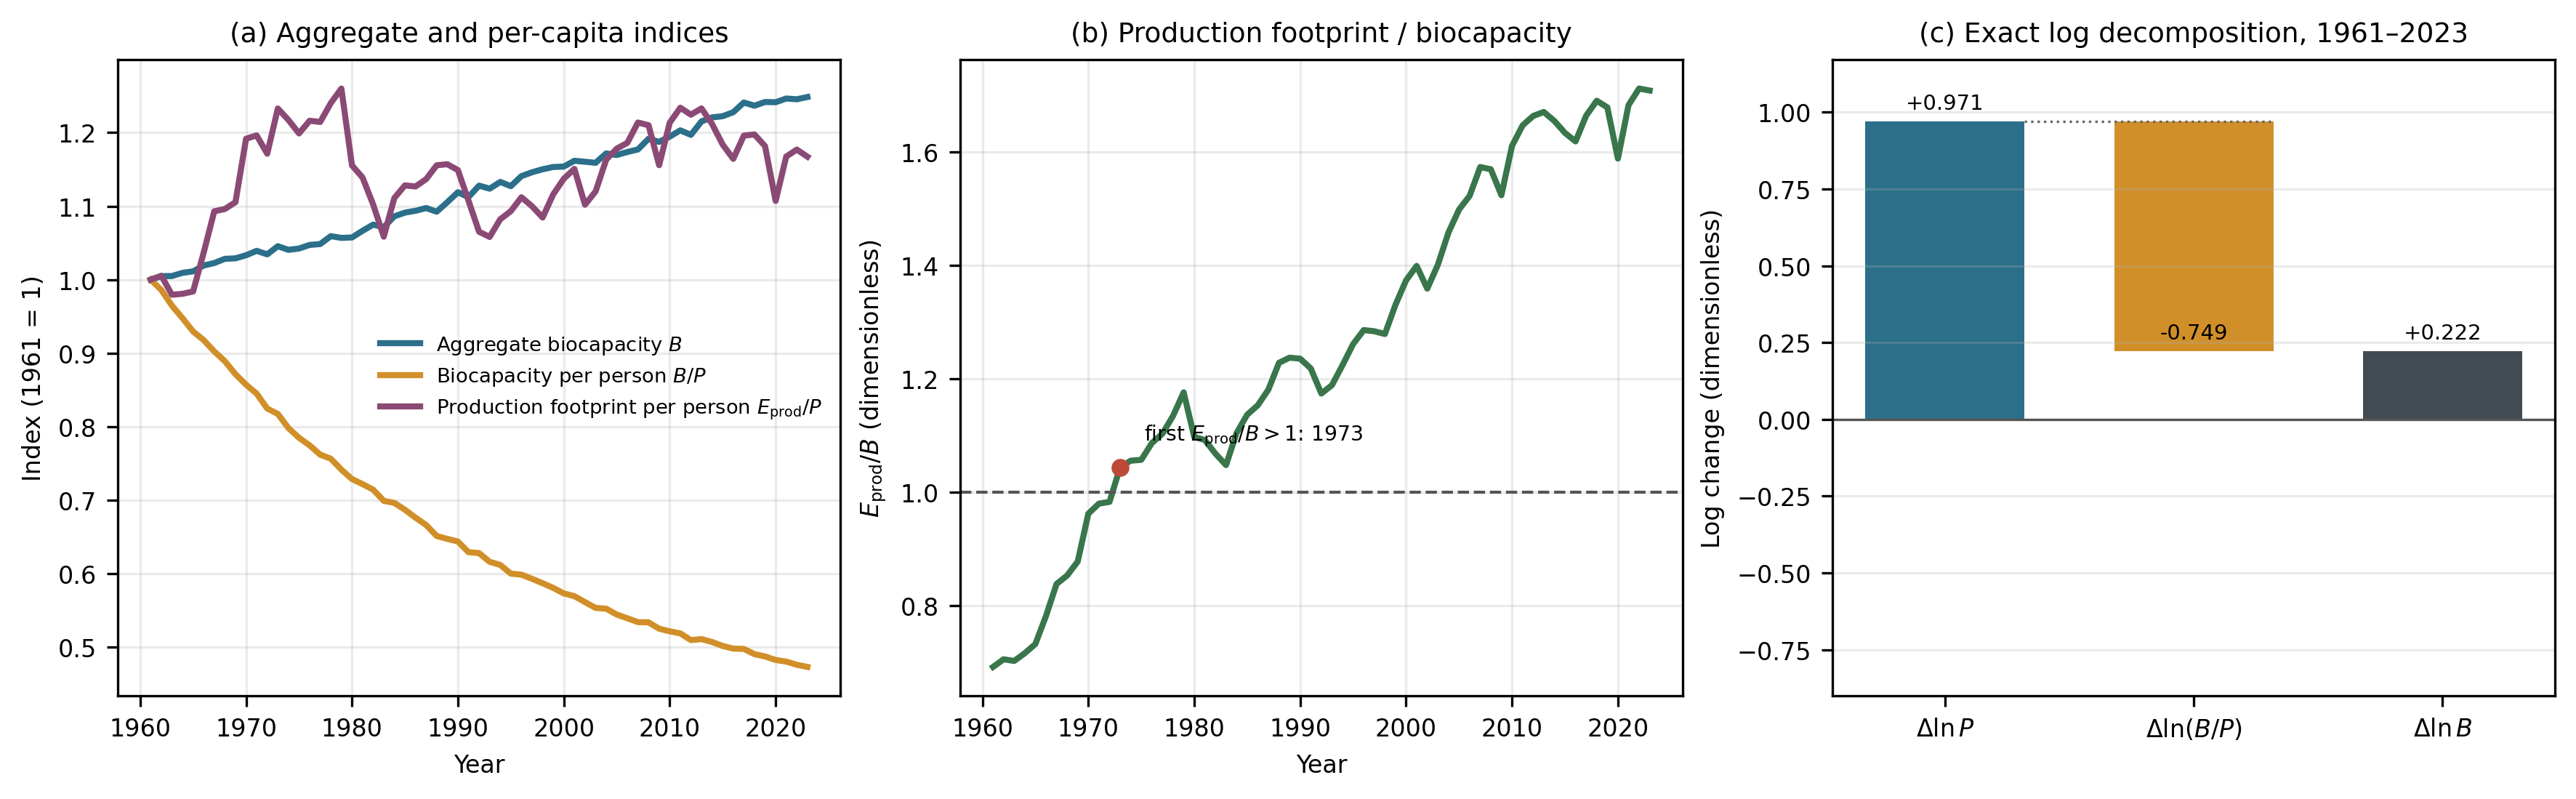
\includegraphics[width=\textwidth]{fig2_nfa_aggregation_face}
\caption{Aggregate and per-capita movements in NFA Edition 2026 (world, 1961--2023; complete observations). $B$ is total biocapacity, $E_{\mathrm{prod}}$ is the workbook's Global Ecological Footprint of Production, and $P$ is the single UN PopStat population series; per-capita values are calculated from totals. (a) Indices (1961 $=1$) of $B$, $B/P$, and $E_{\mathrm{prod}}/P$. (b) $E_{\mathrm{prod}}/B$, first above one in 1973. (c) Exact log identity $\Delta\ln B=\Delta\ln P+\Delta\ln(B/P)$. Account values are in gha; plotted indices, ratios, and log changes are dimensionless. The 2024--2025 estimated rows are excluded.}
\label{fig:aggregation}
\end{figure}

The component series show how NFA account composition changed (Fig.~\ref{fig:composition}; Table~\ref{tab:nfa_components}). Cropland contributes $+24.06$ percentage points to the aggregate's $+24.86\%$ change—about $96.8\%$ of the net percentage change. \mbox{Forest biocapacity} contributes $-5.95$ points, grazing land $-0.27$, fishing grounds $-0.42$, and built-up land $+7.44$. The non-cropland account sum, which includes built-up land, is nearly unchanged ($1.0092\times$, or $+0.80$ points) because the built-up increase offsets declines elsewhere. These are changes in account values. They do not establish changes in forest biomass, soil condition, wetland extent, fish biomass, or model area $A_c$. Built-up land is an account class, not ecological capital. Component values sum to total biocapacity within workbook rounding at both endpoints.

\begin{table}[!htbp]
\centering\footnotesize
\caption{NFA Edition 2026 biocapacity-account endpoint ratios and contributions. Contributions are $100\,[B_i(T)-B_i(1961)]/B(1961)$ percentage points; endpoint ratios are $B_i(T)/B_i(1961)$. The 2022 sensitivity is from the same edition. All entries are account values, not physical-stock measurements.}
\label{tab:nfa_components}
\begin{tabularx}{\textwidth}{@{}Xrrrr@{}}
\toprule
Component & \shortstack{2023\\ratio} & \shortstack{2023 contribution\\(pp of $B_{1961}$)} & \shortstack{2022 sensitivity\\ratio} & \shortstack{2022 contribution\\(pp of $B_{1961}$)} \\
\midrule
Cropland & 2.8701 & $+24.0577$ & 2.8514 & $+23.8183$ \\
Grazing land & 0.9828 & $-0.2688$ & 0.9815 & $-0.2890$ \\
Forest biocapacity & 0.8996 & $-5.9525$ & 0.9019 & $-5.8137$ \\
Fishing grounds & 0.9627 & $-0.4212$ & 0.9596 & $-0.4559$ \\
Built-up land$^{\dagger}$ & 8.7935 & $+7.4416$ & 8.6298 & $+7.2854$ \\
Non-cropland sum$^{\dagger}$ & 1.0092 & $+0.7990$ & 1.0083 & $+0.7267$ \\
\midrule
Total biocapacity & 1.2486 & $+24.8568$ & 1.2454 & $+24.5450$ \\
\bottomrule
\end{tabularx}
\begin{flushleft}\footnotesize
$^{\dagger}$Built-up land is not ecological capital; the non-cropland account sum includes it. Component sums match total biocapacity within workbook rounding. \end{flushleft}
\end{table}

\begin{figure}[!htbp]
\centering
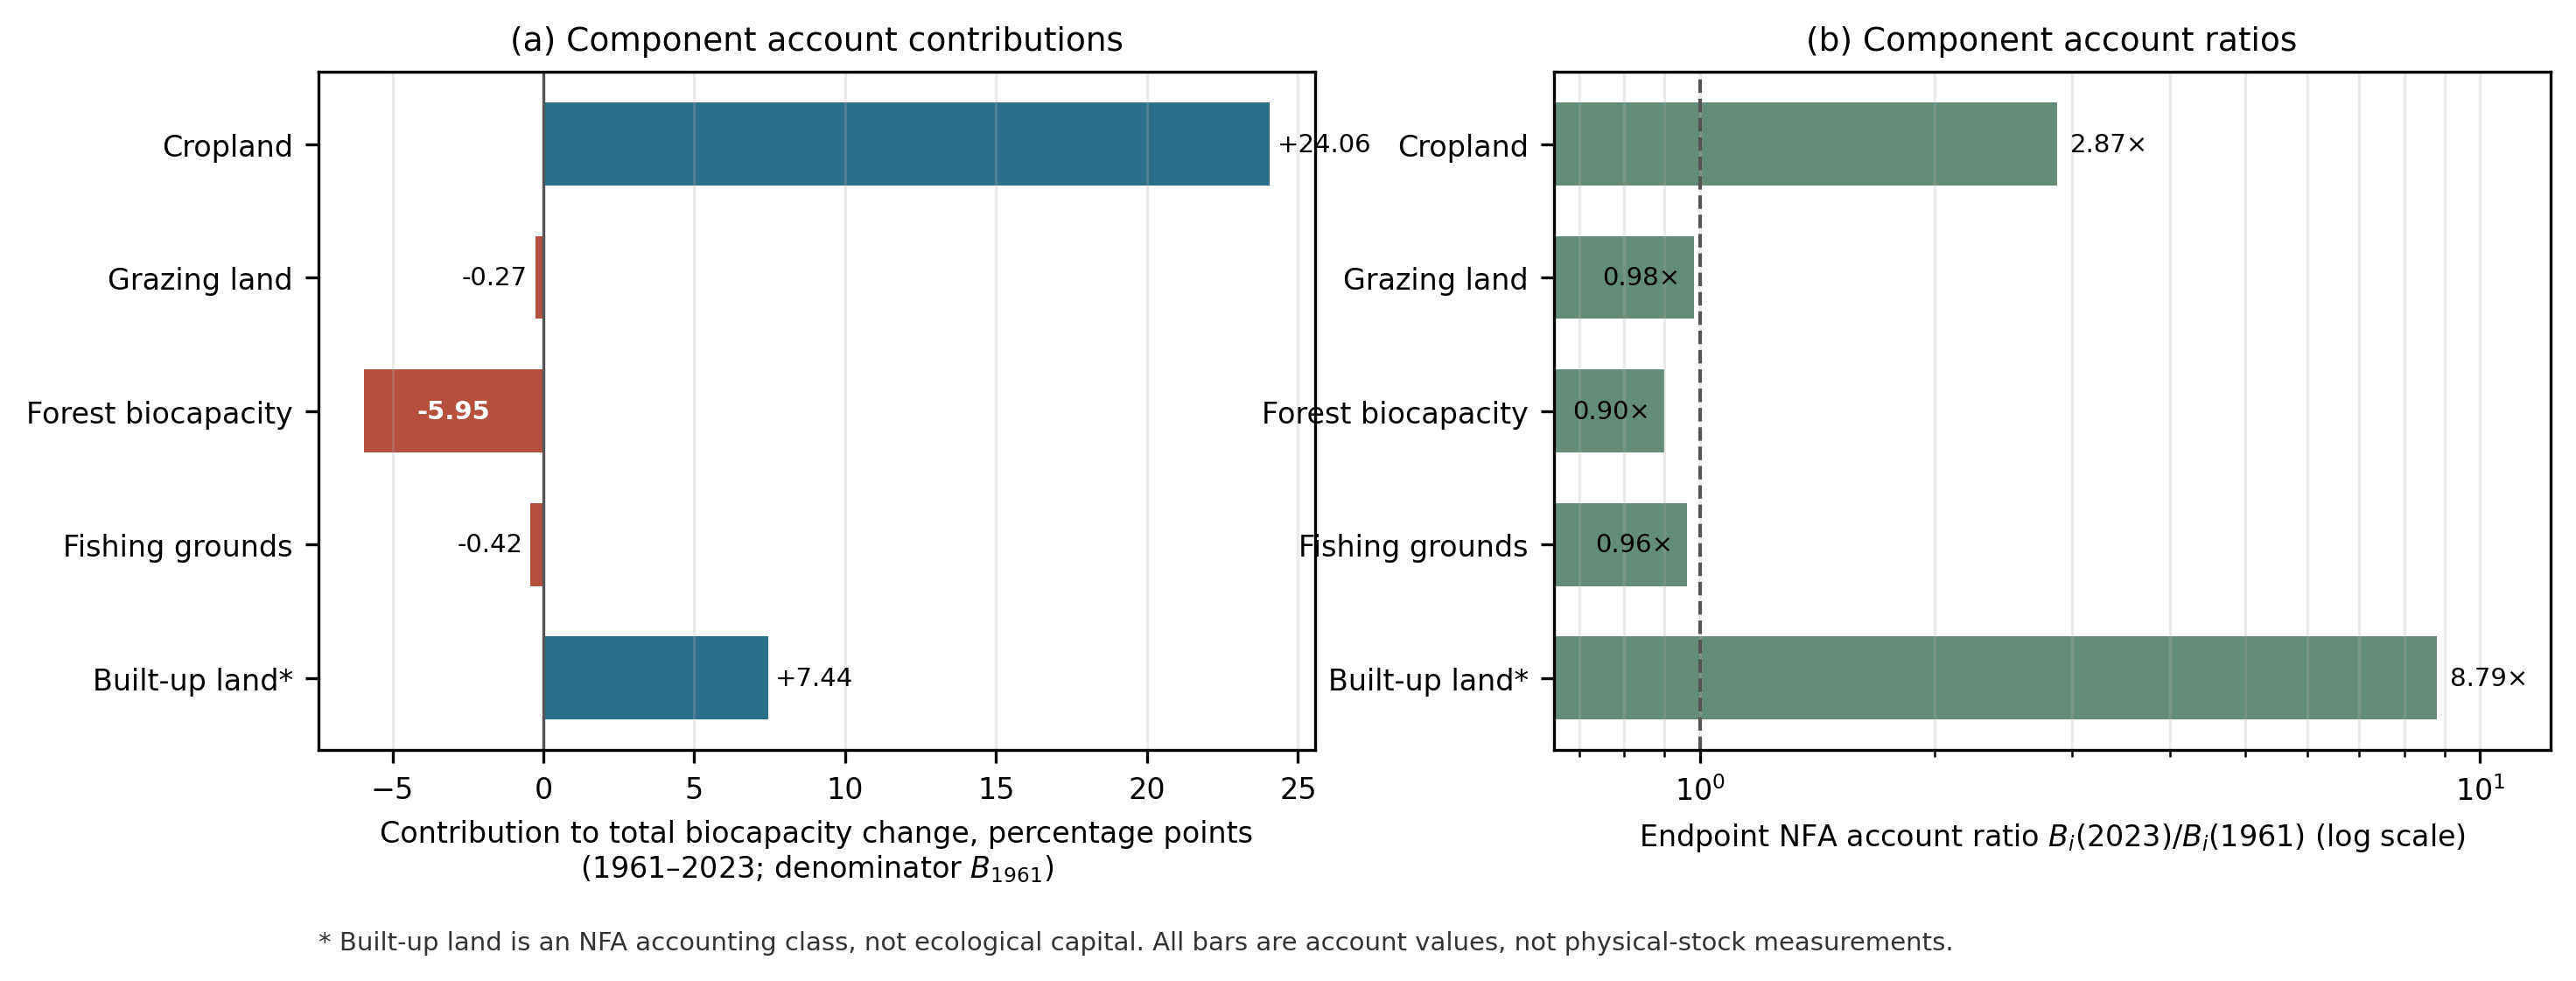
\includegraphics[width=0.95\textwidth]{fig3_composition_attribution}
\caption{NFA Edition 2026 land-type biocapacity-account changes, world, 1961--2023. (a) Component contributions in percentage points of $B_{1961}$. (b) Endpoint ratios $B_i(2023)/B_i(1961)$. “Forest biocapacity” is the workbook's exact label. All bars are account values, not measurements of physical stocks; built-up land is an NFA accounting class, not ecological capital.}
\label{fig:composition}
\end{figure}

We also use external cropland area and cereal yield to build an illustrative proxy for the fast-land contribution (SI~\S S5). Anchoring it to the measured 1961 NFA cropland share ($\phi_0=0.128647$, about $12.86\%$), the exact log-change split assigns $+0.268662$ to the cereal-yield index, $+0.037710$ to cropland area, and $-0.084375$ to the residual. Together these sum to $\Delta\ln B=+0.221997$. The identity is exact for this proxy, but its allocation changes with the anchor and is not a physical-stock attribution.

\subsection{Falsifiable predictions}\label{sec:predictions}

The model yields five testable predictions. Aggregate $B$ alone cannot test them: the composition mechanism requires independent observations or defensible proxies for $A_c$, fast-land area, and yield; testing delay, recovery, and demand-threshold predictions also requires relevant time series and intervention or demographic data.
\begin{enumerate}[label=P\arabic*.,leftmargin=2.2em]
\item \textbf{Conversion can raise the total under a specific condition.} In the baseline frozen-demand run, $\dot A_c<0$ while $\dot B>0$ for a finite interval (Fig.~\ref{fig:model}a). Conversion adds to $B$ exactly when $\dconv>0$, although other flows, quality, debt, technology, and restoration determine the net change. With baseline shares $\sigma_f=\sigma_c=1$, conversion requires demand to exceed total biocapacity ($R_B=E/B>1$). The reserved-share extension can permit conversion when $R_B\le1$, but that is not a baseline result. A composition mask is rising $B$ with falling $A_c$; a liquidation mask is steady $E$ with falling $A_c$. The two patterns may overlap but are not interchangeable. The sign of $\dconv$ describes conversion's contribution, not necessarily the net change in $B$.
\item \textbf{The duration depends on model rates, not a universal horizon.} The slow return rate $\lambda_1$ (along with $\tconv$, $\mu$, $\eta_f$, and $b_c/b_f$) sets the timescale; $\dconv$ and the initial shortfall affect the size of the change. In the baseline, most conversion occurs within one to two e-folding times, when the remaining gap shrinks by a factor of $e$.
\item \textbf{The reduced model has no fold-type early warning.} Return time does not grow as demand approaches the ceiling, and drawdown depth changes continuously with demand (Fig.~\ref{fig:model}c). The model instead signals that $A_c$ is approaching its minimum. It predicts no fold-related warning before that boundary.
\item \textbf{The baseline 20/40-year comparison is saturation-induced.} At $q(s)=0.9$, $\rho_c=0.08$\,yr$^{-1}$ and $q_{\max}=1$, the projected quality reaches its imposed ceiling at $125/9\approx13.8889$\,yr, before either $\tau_g=20$ or $40$\,yr elapses. Those quality paths and matched outcomes therefore coincide; the $\tau_g=5$\,yr case is distinct. The finite comparison does not establish general delay robustness (SI Table S2).
\item \textbf{Recovery requires a return flow.} Lower demand alone does not restore capital-land area. The model needs an explicit restoration flow. A surplus-gated flow is inactive during shortfall, whereas a deficit-gated flow can further reduce provision.
\end{enumerate}
\clearpage
